\section{Evaluation}
\label{sec:eval}

\subsection{Evaluation setting}
\label{sec:setup}

\textbf{Research questions.}
\textbf{RQ1} How accurate is \nscg compared with PyCG-2021 and PyCG-2026?
\textbf{RQ2} What does each component of \nscg contribute, and how much does the
model matter?
\textbf{RQ3} Which edges does each approach get wrong, and why?
\textbf{RQ4} Do the LLM's answers depend on memorised names, and are they stable
across runs?
\textbf{RQ5} Do hybrids of PyCG and \nscg combine their strengths?

\textbf{Subjects.} We use the two benchmarks of the PyCG evaluation repository~\cite{pycgeval2026}
(commit \texttt{8a2e52c}), because they are the only Python call-graph
benchmarks with executable baselines and carefully defined ground truths.
(i) The \emph{micro-benchmark}: the 622 cases up to Python~3.12 (the cohort the
evaluation uses to compare tools), small programs of 34 feature categories
(classes, decorators, dynamic features, imports, standard library, \dots), each
with a ground truth validated against a dynamic trace. (ii) Four packages of the
\emph{macro-benchmark} (Table~\ref{tab:subjects}), whose ground truths are
call-site ledgers written by hand, checked against the traces of the packages'
test suites, and audited four times. Given a limited budget and the course's
guidance of three to four real projects, we selected them to cover both regimes
of the baseline: two where PyCG-2026 is strong (autojump, a small script-like
utility; jmespath, an interpreter with visitor dispatch through
\texttt{getattr}) and two where it is weak (fabric, which subclasses and is
called back by the Invoke framework; funcy, a higher-order functional library),
two from the ICSE~2021 set and two from later batches.

\begin{table}[t]
  \caption{The four packages (sources at the pinned commits of the benchmark).
  Edges in/out: ground-truth edges inside / outside the package. Sites: call
  sites found by the \nscg front-end.}
  \label{tab:subjects}
  \small
  \setlength{\tabcolsep}{3.2pt}
  \begin{tabular}{l l r r r r r r}
\toprule
Package & batch & LOC & mod. & nodes & edges in/out & sites & PyCG F1\\
\midrule
autojump & ICSE'21 & 488 & 3 & 46 & 35/100 & 139 & 0.95 \\
fabric & ICSE'21 & 2,303 & 12 & 93 & 99/252 & 377 & 0.71 \\
jmespath & 1 & 1,675 & 8 & 190 & 310/120 & 470 & 0.99 \\
funcy & 5 & 2,392 & 16 & 305 & 511/475 & 987 & 0.65 \\
\bottomrule
\end{tabular}

\end{table}

\textbf{Criteria.} Edge precision, recall and $F_1$, computed by the official
scorer (\texttt{evaluation/common/score.py}, raw names) separately for callees
inside the package (the headline, as in the PyCG evaluation) and outside it; for
the micro-benchmark also the number of cases whose graph equals the ground truth
exactly. A run that fails counts every edge of its program as missed.

\textbf{Setup.} All runs use one machine (Ubuntu 22.04, 128 cores, 755\,GB
RAM) and Python~3.14.3. The baselines run through the official runner with a
30-minute and 16\,GiB limit per program (PyCG-2021 timed out on funcy, as in
the PyCG evaluation). \nscg uses Claude Haiku~5.5 (and Sonnet~5.5 for RQ2)
through \texttt{claude -p} 2.1.321, 16 requests in parallel, default sampling
(the CLI exposes no temperature), one sample per request; RQ4 repeats the
macro runs with independent samples. The same subjects, entry points and
package roots are given to every tool, and no tool sees the ground truth. The
skill text of the prompts was written from the benchmark's documented
conventions (the same information the PyCG authors had), and the prompts were
developed on a handful of micro cases only; the four packages were not used to
tune the prompts before the V2 run. The total LLM cost of every request of the
study is US\$21.15 (Table~\ref{tab:cost}), of which the
Sonnet runs are three quarters. Money was not the binding constraint; the time
frame of the project (one week of wall-clock time, including the 30-minute
limits of the baselines) and the course's guidance limited the macro
evaluation to four packages, and we chose the cheapest model as the default so
that every variant could be run on all subjects.


\begin{table*}[t]
  \caption{Accuracy of every tool (official scorer, raw names). Inside: edges
  whose callee is in the analysed package (the headline); outside: edges to
  builtins, the standard library and other packages; exact: micro cases whose
  graph equals the ground truth. Bold: best single tool in a column. All \nscg
  variants use Haiku~5.5; Sonnet rows are discussed in RQ2. PyCG-2021 timed out
  on funcy (all its edges count as missed).}
  \label{tab:main}
  \small
  \setlength{\tabcolsep}{3.6pt}
  \begin{tabular}{l rrr rr r rrr rrr}
\toprule
& \multicolumn{6}{c}{Micro-benchmark (622 cases)} & \multicolumn{6}{c}{Four packages (1,973 sites)}\\
\cmidrule(lr){2-7}\cmidrule(lr){8-13}
& \multicolumn{3}{c}{inside} & \multicolumn{2}{c}{outside} & & \multicolumn{3}{c}{inside} & \multicolumn{3}{c}{outside}\\
\cmidrule(lr){2-4}\cmidrule(lr){5-6}\cmidrule(lr){8-10}\cmidrule(lr){11-13}
Tool & P & R & F1 & P & R & exact & P & R & F1 & P & R & F1\\
\midrule
PyCG-2021 (baseline) & 0.868 & 0.605 & 0.713 & 0.862 & 0.660 & 201 & 0.927 & 0.308 & 0.462 & 0.869 & 0.288 & 0.432 \\
PyCG-2026 (baseline) & 0.925 & 0.936 & 0.931 & \textbf{0.996} & 0.962 & \textbf{466} & 0.894 & 0.712 & 0.793 & 0.879 & 0.827 & 0.852 \\
\midrule
S1 only (no LLM) & 0.891 & 0.606 & 0.721 & 0.906 & 0.850 & 118 & 0.963 & 0.550 & 0.700 & 0.891 & 0.714 & 0.792 \\
V0 LLM-only & 0.893 & \textbf{0.995} & \textbf{0.941} & 0.956 & 0.829 & 265 & 0.958 & 0.685 & 0.799 & 0.965 & 0.764 & 0.853 \\
V1 sites, no hints & 0.903 & 0.969 & 0.935 & 0.938 & 0.949 & 258 & 0.967 & 0.703 & 0.814 & 0.915 & 0.826 & 0.868 \\
V2 NSCG & 0.892 & 0.974 & 0.932 & 0.931 & 0.939 & 251 & 0.912 & 0.730 & 0.811 & 0.880 & 0.846 & 0.863 \\
V2.1 NSCG (final) & 0.889 & 0.974 & 0.930 & 0.929 & 0.939 & 251 & 0.913 & 0.732 & 0.812 & 0.899 & 0.859 & 0.879 \\
V3 hybrid (V2+PyCG) & -- & -- & -- & -- & -- & -- & 0.923 & 0.729 & 0.815 & 0.898 & 0.864 & 0.880 \\
V3 hybrid (V2.1+PyCG) & -- & -- & -- & -- & -- & -- & 0.923 & 0.729 & 0.815 & 0.917 & 0.874 & \textbf{0.895} \\
\midrule
PyCG-2026 $\cup$ V2.1 & 0.875 & 0.994 & 0.931 & 0.932 & 0.989 & 428 & 0.844 & 0.746 & 0.792 & 0.831 & 0.902 & 0.865 \\
PyCG-2026 $\cap$ V2.1 & 0.943 & 0.916 & 0.929 & 0.995 & 0.911 & 450 & 0.977 & 0.698 & 0.814 & 0.967 & 0.784 & 0.866 \\
\midrule
V0 LLM-only, Sonnet & -- & -- & -- & -- & -- & -- & 0.944 & 0.619 & 0.748 & 0.974 & 0.753 & 0.849 \\
V2.1 NSCG, Sonnet & 0.912 & 0.973 & 0.941 & 0.930 & 0.926 & 273 & 0.928 & 0.739 & 0.823 & 0.950 & 0.822 & 0.882 \\
\bottomrule
\end{tabular}

\end{table*}

\subsection{RQ1: accuracy against the symbolic baselines}
\label{sec:rq1}

Table~\ref{tab:main} and Figure~\ref{fig:pr} give the aggregate results, and
Table~\ref{tab:projects} the results per package.

\textbf{Four packages.} The final design V2.1 reaches inside
P\,\R{macro-ins-p-nscg-v21} / R\,\R{macro-ins-r-nscg-v21} /
$F_1$\,\R{macro-ins-f1-nscg-v21}, against \R{macro-ins-p-pycg-2026} /
\R{macro-ins-r-pycg-2026} / \R{macro-ins-f1-pycg-2026} for PyCG-2026: slightly
higher precision and recall in aggregate, but not uniformly, and the
aggregate gap ($+$0.019 $F_1$) is only about twice the run-to-run standard deviation of
\nscg (RQ4), so we read it as parity. \nscg is better on autojump
(PyCG-2026 reports four lambdas that the functions only hand to lazy
\texttt{map}/\texttt{filter} objects returned to the caller, which the
callback rule attributes to the caller; \nscg gets all 35 edges right) and on
funcy, slightly better on jmespath, and on fabric it trades precision
(\R{fabric-in-p-nscg-v21} vs.\ \R{fabric-in-p-pycg-2026}) for recall
(\R{fabric-in-r-nscg-v21} vs.\ \R{fabric-in-r-pycg-2026}). PyCG-2021 is far
behind (inside $F_1$ \R{macro-ins-f1-pycg-2021}): it misses most edges through
library values and timed out on funcy (even without funcy its recall on the other
three packages is clearly lower, Table~\ref{tab:projects}). On outside edges \nscg also leads
($F_1$ \R{macro-out-f1-nscg-v21} vs.\ \R{macro-out-f1-pycg-2026}).

\textbf{Micro-benchmark.} The picture is different. Every LLM-based variant has
a much higher inside recall than PyCG-2026 (V2.1 \R{micro-ins-r-nscg-v21}, V0
\R{micro-ins-r-llm-only} vs.\ \R{micro-ins-r-pycg-2026}) but a lower precision
(\R{micro-ins-p-nscg-v21} vs.\ \R{micro-ins-p-pycg-2026}), so the inside $F_1$
values are close, while PyCG-2026 is clearly better on outside names
(P\,\R{micro-out-p-pycg-2026} vs.\ \R{micro-out-p-nscg-v21}) and produces the
exact graph for \R{micro-exact-pycg-2026} of 622 cases against
\R{micro-exact-nscg-v21} for V2.1. The LLM variants are \emph{less exact but
more complete}: they rarely miss a call, but they add plausible edges that the
precise semantics excludes and spell outside callees differently.
Figure~\ref{fig:categories} shows where the tools differ most. The LLM-based
variants win on \emph{dynamic} features (\texttt{eval} of a constructed string,
\texttt{getattr}/\code{operator.methodcaller}, \code{sys.modules}, monkey
patching), on the standard library, on context managers and on missing external
modules --- cases where reading the code as a developer does beats an
abstraction; PyCG-2026 wins on exactly specified semantics: tuples, strings,
\texttt{match}, argument binding, async code and class hierarchies.

\begin{figure*}[t]
  \centering
  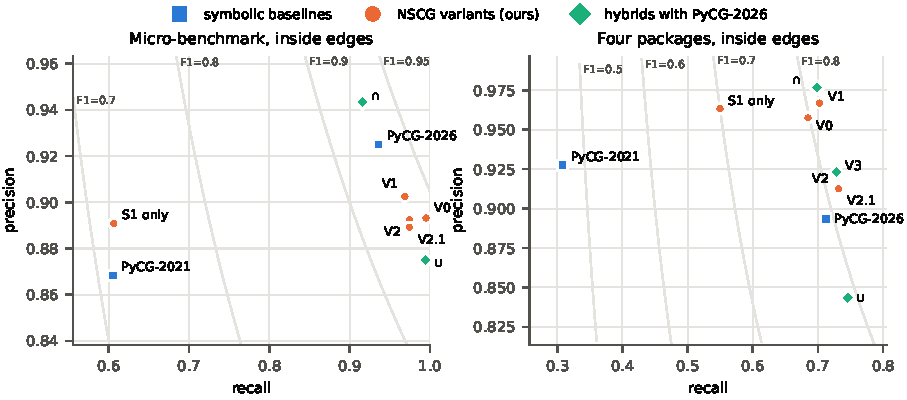
\includegraphics[width=0.86\textwidth]{figures/pr.pdf}
  \caption{Precision and recall of inside edges; grey lines are $F_1$
  iso-curves. Left: micro-benchmark; right: the four packages (PyCG-2021 timed
  out on funcy, whose edges count as missed).}
  \label{fig:pr}
\end{figure*}

\begin{table*}[t]
  \caption{Inside edges per package (P / R / $F_1$). PyCG-2021 timed out on funcy.}
  \label{tab:projects}
  \small
  \setlength{\tabcolsep}{3.4pt}
  \begin{tabular}{l rrr rrr rrr rrr }
\toprule
& \multicolumn{3}{c}{autojump} & \multicolumn{3}{c}{fabric} & \multicolumn{3}{c}{jmespath} & \multicolumn{3}{c}{funcy}\\
\cmidrule(lr){2-4}\cmidrule(lr){5-7}\cmidrule(lr){8-10}\cmidrule(lr){11-13}
& P & R & F1 & P & R & F1 & P & R & F1 & P & R & F1\\
\midrule
PyCG-2021 & 1.00 & 0.89 & 0.94 & 0.92 & 0.46 & 0.62 & 0.92 & 0.70 & 0.79 & \multicolumn{3}{c}{timeout} \\
PyCG-2026 & 0.90 & 1.00 & 0.95 & 0.96 & 0.56 & 0.71 & 0.97 & 1.00 & 0.99 & 0.81 & 0.55 & 0.65 \\
S1 only & 1.00 & 0.89 & 0.94 & 0.96 & 0.47 & 0.64 & 1.00 & 0.72 & 0.83 & 0.93 & 0.44 & 0.60 \\
V0 & 1.00 & 1.00 & 1.00 & 0.84 & 0.62 & 0.71 & 1.00 & 1.00 & 1.00 & 0.94 & 0.49 & 0.64 \\
V2 & 1.00 & 1.00 & 1.00 & 0.88 & 0.62 & 0.73 & 1.00 & 0.99 & 1.00 & 0.83 & 0.57 & 0.68 \\
V2.1 & 1.00 & 1.00 & 1.00 & 0.89 & 0.64 & 0.74 & 1.00 & 0.99 & 1.00 & 0.83 & 0.57 & 0.68 \\
V3 (V2.1) & 1.00 & 0.89 & 0.94 & 0.89 & 0.64 & 0.74 & 1.00 & 1.00 & 1.00 & 0.86 & 0.57 & 0.69 \\
$\cup$ & 0.90 & 1.00 & 0.95 & 0.89 & 0.64 & 0.74 & 0.97 & 1.00 & 0.99 & 0.73 & 0.60 & 0.66 \\
\bottomrule
\end{tabular}

\end{table*}

\begin{figure}[t]
  \centering
  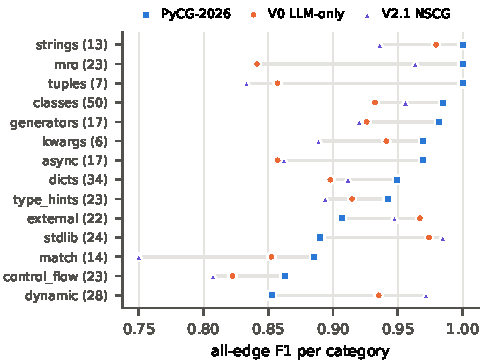
\includegraphics[width=0.95\columnwidth]{figures/categories.pdf}
  \caption{All-edge $F_1$ per micro category (number of cases in parentheses)
  for the 14 categories where PyCG-2026, V0 and V2.1 differ most.}
  \label{fig:categories}
\end{figure}

\subsection{RQ2: what each component contributes}
\label{sec:rq2}

\textbf{The symbolic front-end alone} (S1 only) is precise but incomplete:
inside P\,\R{macro-ins-p-nscg-sym} but R\,\R{macro-ins-r-nscg-sym} on the
packages, recall \R{micro-ins-r-nscg-sym} on micro. Its resolver is deliberately
cheap; it is not meant to be an analysis of its own, yet it already matches
PyCG-2021's micro accuracy (all-edge $F_1$ \R{micro-all-f1-nscg-sym} vs.\
\R{micro-all-f1-pycg-2021}).

\textbf{The LLM alone} (V0) is a strong baseline --- one of the main surprises
of the study. On the packages it has higher precision than V2.1
(\R{macro-ins-p-llm-only}) but lower recall (\R{macro-ins-r-llm-only}); on
micro it has the best inside recall of all single tools. Its weaknesses are
systematic rather than random: it omits calls that are easy to overlook in a
whole-program answer (V0 loses most of its micro \emph{mro} points by omitting the
\code{<builtin>.super} edge that every \texttt{super()} call creates, which
\nscg's site enumeration never misses), it names outside callees less
consistently, and it cannot be checked.

\textbf{Per-site hints} (V1$\rightarrow$V2) are a double-edged sword. With the
same sites but no symbolic information, V1 is the most \emph{precise}
LLM variant on the packages (P\,\R{macro-ins-p-nscg-nohints}, R\,\R{macro-ins-r-nscg-nohints});
adding resolutions, name candidates, callbacks and facts raises recall to
\R{macro-ins-r-nscg} but lowers precision to \R{macro-ins-p-nscg}, so $F_1$ is
unchanged (\R{macro-ins-f1-nscg-nohints} vs.\ \R{macro-ins-f1-nscg}). The model
tends to \emph{accept} plausible candidates: 57 of V2's inside false
positives were proposed by the front-end (Table~\ref{tab:errors}), most of them
name matches in funcy (e.g.\ every \code{__getitem__} of the package at a
subscript of an unknown mapping).

\textbf{The validator} turned out to be nearly neutral (a negative result).
Given the outline and the candidates, the model rarely invents package names:
on the packages it added only \R{err-fp-llm-added-nscg-v21} wrong package
callees that no component proposed, and the validator rejected a single unknown
package name in V2.1 (Table~\ref{tab:validation}). Without any validation (raw
names), V2.1 scores inside $F_1$ \R{macro-ins-f1-nscg-v21-novalidate} and
outside $F_1$ \R{macro-out-f1-nscg-v21-novalidate}, i.e.\ the same as with it.
V2's alias expansion was in fact \emph{harmful} (outside $F_1$
\R{macro-out-f1-nscg}); the three fixes of V2.1 only removed that harm. The
symbolic floor is slightly harmful on micro (exact cases
\R{micro-exact-nscg-v21} with it, \R{micro-exact-nscg-v21-nofloor} without;
Section~\ref{sec:discussion}).

\textbf{Library hooks and the model.} With Haiku, the library hooks of V2.1
recovered only two Fabric edges: at \texttt{self.\_run(runner, command)} in
\code{Connection.run}, the prompt listed the methods of Fabric's
\texttt{Remote} runner that Invoke's \code{Runner.run} calls back, but Haiku
kept only \code{invoke.Context._run}. With Sonnet~5.5 and the same prompt,
the model used its knowledge of Invoke and recovered 18 of these callbacks
(\code{Connection.run}/\texttt{sudo} $\rightarrow$ \code{Remote.start},
\code{read_proc_stdout}, \code{send_interrupt}, \dots), raising Fabric's
recall from \R{fabric-in-r-nscg-v21} to \R{fabric-in-r-nscg-v21@sonnet}. Overall,
Sonnet improves V2.1 moderately (inside $F_1$ \R{macro-ins-f1-nscg-v21@sonnet}
on the packages, \R{micro-ins-f1-nscg-v21@sonnet} on micro) at about ten times
the cost. As an LLM-only analyzer, however, Sonnet is \emph{worse} than Haiku
(\R{macro-ins-f1-llm-only@sonnet} vs.\ \R{macro-ins-f1-llm-only}), mainly through
lower recall (jmespath \R{jmespath-in-r-llm-only@sonnet}): the structure that
\nscg imposes matters more than the model.

\begin{table}[t]
  \caption{Decisions of the validator S2 (callee names over all sites): package / outside names kept,
  unknown package names rejected, \texttt{C.\_\_init\_\_} mapped to the constructor through the MRO,
  and certain symbolic resolutions added by the floor. The other rules (path repair, class$\to$constructor,
  inherited$\to$definer, outside names at implicit sites, and V2.1's \texttt{builtins.X} renaming) never fired.}
  \label{tab:validation}
  \small
  \setlength{\tabcolsep}{4pt}
  \begin{tabular}{l l rrrrr}
\toprule
Run & bench. & kept in & kept out & rejected & init$\to$ctor & floor\\
\midrule
V2 & micro & 1438 & 490 & 5 & 2 & 18 \\
V2 & macro & 928 & 1093 & 3 & 0 & 16 \\
V2.1 & micro & 1444 & 493 & 5 & 2 & 16 \\
V2.1 & macro & 930 & 1095 & 1 & 0 & 5 \\
V1 & micro & 1405 & 489 & 1 & 0 & 28 \\
V1 & macro & 843 & 1034 & 12 & 0 & 16 \\
\bottomrule
\end{tabular}

\end{table}


\subsection{RQ3: successes and failures}
\label{sec:rq3}

Table~\ref{tab:errors} labels every false negative and false positive on the
four packages. The labels use what the front-end proposed at the sites of the
caller.

\begin{table*}[t]
  \caption{Error taxonomy on the four packages. FN inside: \emph{no hint} -- no
  site of the caller proposed the callee; \emph{dropped} -- proposed but
  dropped by the LLM. FN outside: \emph{misnamed} -- the tool has an outside
  callee of the same caller with the same last name component. FP inside:
  \emph{from hint} -- proposed by the front-end and kept; \emph{added} -- added
  by the LLM. FP outside: \emph{misnamed} -- the ground truth has a callee with
  the same last component.}
  \label{tab:errors}
  \small
  \begin{tabular}{l rrrr rrrr}
\toprule
& \multicolumn{4}{c}{false negatives} & \multicolumn{4}{c}{false positives}\\
\cmidrule(lr){2-5}\cmidrule(lr){6-9}
& \multicolumn{2}{c}{inside} & \multicolumn{2}{c}{outside} & \multicolumn{2}{c}{inside} & \multicolumn{2}{c}{outside}\\
Tool & no hint & dropped & misnamed & omitted & from hint & added & misnamed & spurious\\
\midrule
S1 only & 389 & 41 & 56 & 215 & 20 & 0 & 63 & 20 \\
V0 & 276 & 25 & 24 & 199 & 16 & 13 & 10 & 16 \\
V2 & 255 & 3 & 64 & 82 & 57 & 10 & 61 & 48 \\
V2.1 & 253 & 3 & 53 & 80 & 57 & 10 & 43 & 48 \\
V3 (V2.1) & 253 & 6 & 53 & 66 & 53 & 5 & 41 & 34 \\
\bottomrule
\end{tabular}

\end{table*}

\textbf{The LLM filters; it rarely discovers.} \R{err-fn-no-evidence-nscg-v21}
of V2.1's \R{macro-ins-fn-nscg-v21} missed inside edges had no hint at any site
of the caller, and only \R{err-fp-llm-added-nscg-v21} inside false positives
were added by the model without a hint. The hints decide what \nscg can find;
the three repetitions of RQ4 have \emph{identical} inside recall. Where the hint
is there, the model is good at keeping the right callees: only
\R{err-fn-rejected-nscg-v21} proposed true edges were dropped.

\textbf{A hard core that no tool finds.} Of V2.1's
\R{macro-ins-fn-nscg-v21} missed inside edges, 243 are also missed by
PyCG-2026 (which misses only 32 inside edges that V2.1 finds). They come from
two mechanisms. (1) \emph{Library callbacks}: Fabric's \code{Connection.run}
hands a \texttt{Remote} runner to Invoke, whose \code{Runner.run} calls back
\texttt{start}, \code{read_proc_stdout}, \code{send_start_message} and
others; the ground truth reads Invoke's code to find them, PyCG-2026 does not
model outside code that calls back, and \nscg's model did not supply the
knowledge. (2) \emph{Documented roles}: funcy's ground truth gives a parameter
such as \texttt{pred} of \code{_lfilter} every package function that the
documentation or the tests pass in that role (\texttt{isnone}, \texttt{even},
the lambdas made by \code{re_tester}, \dots); no tool reads the
documentation, so most of funcy's \R{funcy-in-fn-nscg-v21} missed edges are
of this kind.

\textbf{Where reading beats abstracting.} In jmespath, the metaclass
\code{FunctionRegistry} registers only the methods whose name starts with
\code{_func_}, and \code{call_function} calls the registered function.
PyCG-2026 cannot evaluate the string filter and reports every method of the
class (7 false positives such as \code{_type_check}); \nscg calls only the
\code{_func_} methods. In the micro-benchmark, \nscg resolves
\texttt{eval(measure + "()")} with \texttt{measure = "area"} to
\code{main.area}, and similar string-built dispatches, which PyCG treats as
unknowable by design.

\textbf{Where abstracting beats reading.} PyCG-2026's 466 exact micro graphs
come from strictly applied conventions: it never adds an edge that the
semantics excludes, names every outside callee through typeshed, and handles
argument binding and \texttt{match} precisely. \nscg's micro false positives
are mostly over-approximations accepted from the flow-insensitive hints (a dict
entry overwritten before the call; a lazily built \texttt{map} that is never
consumed) and \emph{misnamed outside callees} (\code{<builtin>.iter.__next__}
for \code{builtins.list_iterator.__next__},
\code{paramiko.transport.Transport.open_session} for the benchmark's access
path \code{paramiko.client.SSHClient.get_transport.open_session}). Of
V2.1's 224 outside errors on the packages, 96 (43\%) are such near misses with
the right last name component (Table~\ref{tab:errors}).

\textbf{Unexpected behaviours.} (i) Evidence can \emph{hurt}: in the hybrid
V3, the model dropped four lambda callbacks of \texttt{autojump} (three in
\code{autojump_data.load}) that both PyCG-2026 and V2 had found and that
PyCG's evidence listed. (ii) The validator itself had bugs that only
the error analysis exposed (the three alias expansions of V2.1). (iii) V0 is
more precise than V2 on the packages, the opposite of what we designed for.

\subsection{RQ4: memorisation and stability}
\label{sec:rq4}

\textbf{Renaming probe.} Both benchmarks are public on GitHub, so the LLM may
have seen the programs, and even the micro-benchmark's ground-truth files. To
test whether its accuracy depends on familiar names, we consistently renamed
every package-defined function and class of the micro cases (to names like
\code{q3f1_0}) where this is syntactically safe, rewrote the ground truth,
and kept the 580 cases whose renamed ground truth the benchmark's own dynamic
validator still accepts. Table~\ref{tab:probe} compares the same 580 cases
before and after renaming.

\begin{table}[t]
  \caption{Renaming probe on 580 micro cases (inside edges; all-edge $F_1$;
  exact cases). Symbolic tools are name-invariant by construction.}
  \label{tab:probe}
  \setlength{\tabcolsep}{3pt}
  \resizebox{\columnwidth}{!}{\begin{tabular}{l rrr rrr rr rr}
\toprule
& \multicolumn{3}{c}{original, inside} & \multicolumn{3}{c}{renamed, inside} & \multicolumn{2}{c}{all-edge F1} & \multicolumn{2}{c}{exact}\\
\cmidrule(lr){2-4}\cmidrule(lr){5-7}\cmidrule(lr){8-9}\cmidrule(lr){10-11}
Tool & P & R & F1 & P & R & F1 & orig. & ren. & orig. & ren.\\
\midrule
PyCG-2026 & 0.924 & 0.946 & 0.935 & 0.924 & 0.946 & 0.935 & 0.946 & 0.946 & 441 & 441 \\
PyCG-2021 & 0.868 & 0.613 & 0.719 & 0.868 & 0.613 & 0.719 & 0.724 & 0.724 & 185 & 185 \\
S1 only & 0.889 & 0.613 & 0.725 & 0.889 & 0.613 & 0.725 & 0.767 & 0.767 & 114 & 114 \\
V0 LLM-only & 0.893 & 0.996 & 0.942 & 0.902 & 0.998 & 0.948 & 0.925 & 0.927 & 261 & 264 \\
V2.1 NSCG & 0.888 & 0.976 & 0.930 & 0.893 & 0.976 & 0.933 & 0.928 & 0.932 & 247 & 255 \\
\bottomrule
\end{tabular}
}
\end{table}

Renaming does not hurt the LLM-based analyzers: V0 goes from inside $F_1$
\R{probe-orig-f1-llm-only} to \R{probe-ren-f1-llm-only} and V2.1 from
\R{probe-orig-f1-nscg-v21} to \R{probe-ren-f1-nscg-v21}, with as many or more
exact cases (V2.1: \R{probe-orig-exact-nscg-v21} $\rightarrow$
\R{probe-ren-exact-nscg-v21}), and the symbolic tools are unchanged, as they
must be. The micro-benchmark results therefore do not depend on recognising
the original identifiers or on recalling the published \code{callgraph.json}
files, whose names no longer match. The probe cannot exclude that the model has
learned the benchmark's \emph{structure} (the cases are small idioms that also
occur everywhere else), and it does not cover the packages, which are too large
to rename safely; we discuss this in Section~\ref{sec:threats}.


\textbf{Stability.} Three independent runs of V2.1 on the packages
(Table~\ref{tab:repeats}) have a standard deviation of \R{repeat-sd-f1} in
inside $F_1$; \R{repeat-agree} edges reported by any run are reported by all
three (\R{repeat-agree-pct}\%). All variation is in precision
(\R{repeat-min-p}--\R{repeat-max-p}, mostly funcy's name-matched
\code{__getitem__} candidates); recall is the same in every run. The differences between the variants in RQ2 that
are smaller than about two standard deviations should therefore not be read
as real effects.

\begin{table}[t]
  \caption{Three runs of V2.1 (Haiku) on the four packages.}
  \label{tab:repeats}
  \small
  \begin{tabular}{l rrr rr}
\toprule
Metric (4 packages) & run 1 & run 2 & run 3 & mean & s.d.\\
\midrule
inside P & 0.913 & 0.890 & 0.936 & 0.913 & 0.023 \\
inside R & 0.732 & 0.732 & 0.732 & 0.732 & 0.000 \\
inside F1 & 0.812 & 0.803 & 0.821 & 0.812 & 0.009 \\
outside P & 0.899 & 0.908 & 0.908 & 0.905 & 0.005 \\
outside R & 0.859 & 0.845 & 0.847 & 0.850 & 0.008 \\
outside F1 & 0.879 & 0.875 & 0.876 & 0.877 & 0.002 \\
\bottomrule
\end{tabular}

\end{table}

\subsection{RQ5: hybrids}
\label{sec:rq5}

The two kinds of analyzers make different false positives (of V2.1's 67 and
PyCG-2026's 81 inside false positives on the packages only 16 are shared) but
largely the same false negatives, so combinations raise precision more easily
than recall. The edge \emph{union} has the highest inside recall on the packages
(\R{macro-ins-r-union--pycg-2026--nscg-v21}) and nearly the highest on micro
(\R{micro-ins-r-union--pycg-2026--nscg-v21}) at a loss of precision; the \emph{intersection} is the most precise configuration
(\R{macro-ins-p-inter--pycg-2026--nscg-v21} / \R{micro-ins-p-inter--pycg-2026--nscg-v21})
and has the best micro inside precision of all. Giving PyCG's callees to the LLM
(V3) yields the best outside $F_1$ (\R{macro-out-f1-nscg-hybrid-v21}) and a
small inside gain (\R{macro-ins-f1-nscg-hybrid-v21}): the model uses PyCG's
typeshed-based outside names, but it does not simply copy PyCG, and the inside
edges that both miss stay missed. A client that needs recall (e.g.\ a
vulnerability reachability check) should use the union; one that needs
precision (e.g.\ refactoring) the intersection.

\subsection{Cost}

Table~\ref{tab:cost} lists every run. A full V2.1 run of the four packages costs
about US\$0.2--0.4 with Haiku and runs in about a minute with 16 parallel
requests; the micro-benchmark costs about US\$0.7. Sonnet costs about ten times
more. PyCG-2026 analyses each package in under a second, at no cost.

\begin{table}[t]
  \caption{LLM usage per run (new requests only; replayed answers are free).}
  \label{tab:cost}
  \small
  \setlength{\tabcolsep}{3pt}
  \begin{tabular}{l rr rr rr}
\toprule
& \multicolumn{2}{c}{micro} & \multicolumn{2}{c}{macro} & \multicolumn{2}{c}{tokens}\\
\cmidrule(lr){2-3}\cmidrule(lr){4-5}\cmidrule(lr){6-7}
Run & req. & USD & req. & USD & in & out\\
\midrule
V2 & 616 & 0.67 & 64 & 0.38 & 2.94M & 516k \\
V0 & 622 & 0.66 & 67 & 0.35 & 2.56M & 589k \\
V1 & 616 & 0.64 & 64 & 0.35 & 2.71M & 525k \\
V3 (V2) & -- & -- & 64 & 0.39 & 0.95M & 222k \\
V2.1 & 7 & 0.01 & 6 & 0.04 & 0.12M & 33k \\
V3 (V2.1) & -- & -- & 6 & 0.04 & 0.10M & 26k \\
V2.1 rep.~2 & -- & -- & 64 & 0.22 & 0.94M & 228k \\
V2.1 rep.~3 & -- & -- & 64 & 0.21 & 0.94M & 211k \\
V2.1 Sonnet & 616 & 7.88 & 64 & 4.39 & 2.97M & 171k \\
V0 Sonnet & -- & -- & 67 & 3.64 & 0.76M & 64k \\
V2.1 renamed & 574 & 0.64 & -- & -- & 1.91M & 306k \\
V0 renamed & 580 & 0.64 & -- & -- & 1.70M & 356k \\
\midrule
\textbf{Total} & \multicolumn{4}{c}{4161 requests, \textbf{US\$21.15}} & 18.6M & 3248k \\
\bottomrule
\end{tabular}

\end{table}
